\chapter{Análisis de Procesos}

\par 
En este capítulo se analizarán dos procesos operativos utilizados por la división de operaciones de la compañía SIGCSA. Los procesos operativos que analizar son los utilizados en campo para la caracterización de medios isotermos y de calibración de termómetros. La compañía SIGCSA nos dio acceso a la documentación correspondiente de cada proceso. Utilizaremos estos procesos como parte de la evaluación de nuestro prototipo.

\section{Proceso Operativo SIGCSA-PO-25}

\par 
El objetivo del proceso es el de proporcionar instrucciones para la caracterización y ajustes (tomando en cuenta las instrucciones
del fabricante) de medios isotermos con el propósito de confirmar el correcto funcionamiento de
la cámara de ensayo de temperatura.\cite{po25}

\par \noindent
La caracterización es el conjunto de operaciones que determinan las diferentes
características metrológicas y especificaciones de operación de un
equipo, instrumento de medición, sistema de medición o medida
materializada. Por lo que este proceso se encarga de obtener las variables metrológicas de un equipo isotérmico, utilizando termómetros en ciertos puntos del equipo.\cite{po25}

\subsection{Alcance}
\par 
Para ser utilizados en Laboratorios Clínicos, de Ensayos, de Investigación y Bancos de Sangre, que
tengan medios isotermos de controles análogos y digitales tales como\cite{po25}:

\begin{itemize}
	\item Refrigerador de 0°C a 6°C (la conservación de sangre y derivados).
	
	\item Refrigerador de 0°C a 8°C (conservación de reactivos).
	
	\item Refrigerador de Baja Temperatura de 0°C a -35°C (conservación de reactivos y derivados
	de la sangre).
	
	\item Refrigerador de Ultra Baja Temperatura 0°C a -80°C (crio preservación de cepas y tejido
	biológico).
	
	\item Incubadoras de -10°C a 75°C (conservación de organismos vivos en un entorno que
	resulte adecuado para su crecimiento y conservación de derivados de la sangre). **
	
	\item Baño de María de temperatura ambiente a 60°C (incubación, inactivación, aglutinación y
	descongelación de derivados de la sangre).
	
	\item Baño Seco de temperatura ambiente a 60°C (incubación).
	
	\item Estufa u Horno de Secado de temperatura ambiente a 100°C (procesos de secado y
	esterilizado de recipientes de vidrio y metal).
\end{itemize}

\begin{figure}[H]
	\centering
	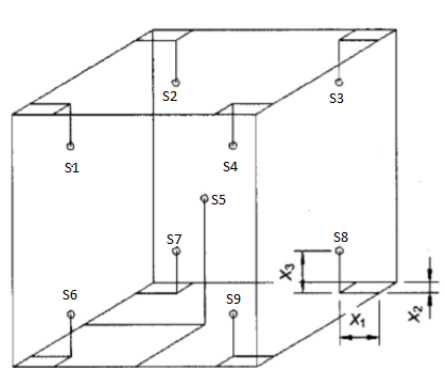
\includegraphics[width=5cm, height=4cm]{isotermo1.png}
	\caption{Medio isotermo 1, capacidad de 50L a 2100L}
\end{figure}

\begin{figure}[H]
	\centering
	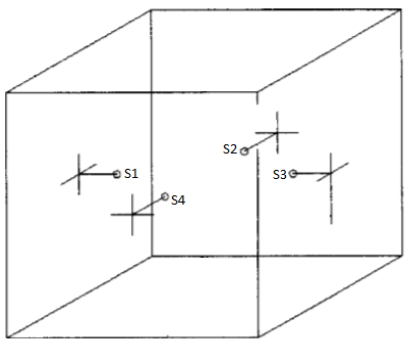
\includegraphics[width=5cm, height=4cm]{isotermo2.png}
	\caption{Medio isotermo 2, capacidad de 2L a 49L}
\end{figure}
	
\subsection{Análisis}


\par \noindent
El procedimiento se puede resumir en 4 pasos:

\begin{itemize}
	\item Preparación: Se determina las incertidumbres de los termómetros utilizados para caracterizar el medio isotermo y para validar que los termómetros se encuentran en buenas condiciones. Se documenta y se valida que las condiciones ambientales donde se encuentra el medio isotérmico son las adecuadas.
	
	\item Instalación: Si todos los parámetros del paso anterior cumplen, entonces procedemos a colocar las sondas, si el medio isotermo tiene una capacidad mayor a 49L se colocan las sondas como en la figura 2.1, en caso contrario como en la figura 2.2
	
	\item Captura de Datos: Se documenta la temperatura y humedad inicial, se captura la información que despliegan los termómetros por el tiempo estipulado en el procedimiento y una vez finalizado el tiempo nuevamente se documenta la temperatura y humedad.
	
	\item Cálculos metrológicos: Una vez capturada la información, se procede a realizar los cálculos que determinarán las características metrológicas del equipo isotérmico. 
\end{itemize}

\begin{figure}[H]
	\centering
	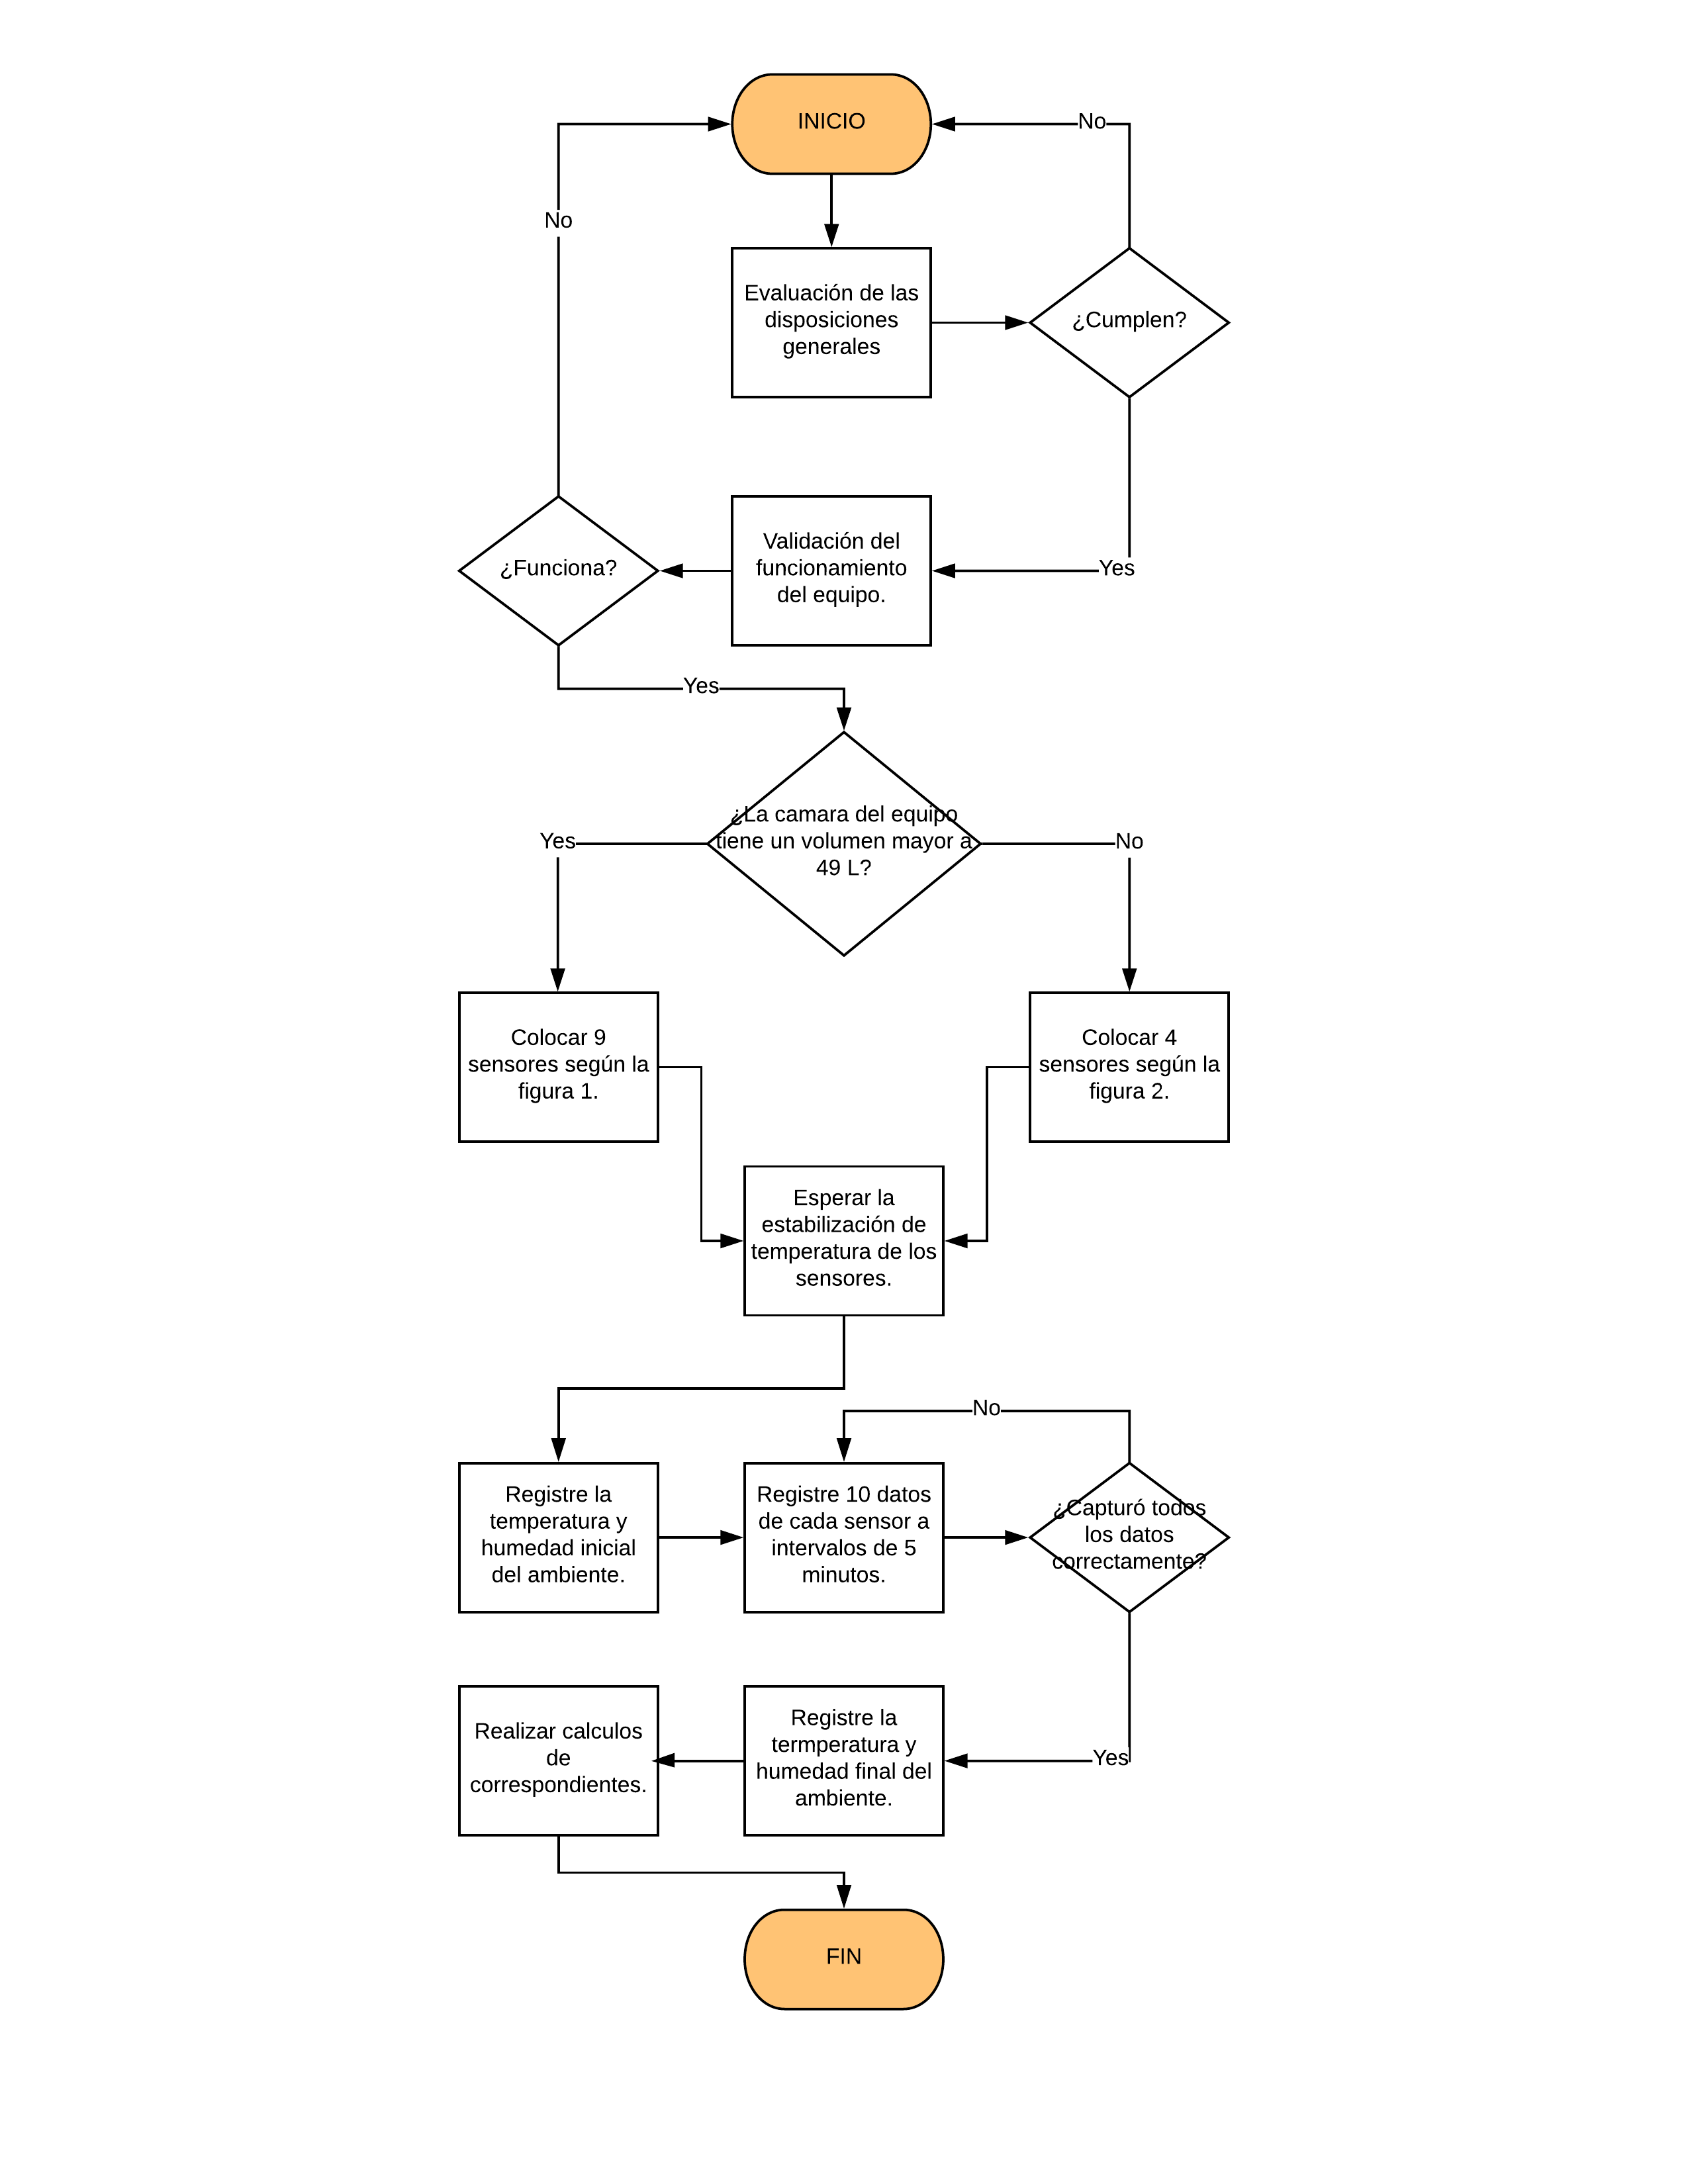
\includegraphics[width=\textwidth]{diagram1.png}
	\caption{Diagrama de flujo del proceso operativo SIGCSA-PO-25}
\end{figure}


\section{Proceso Operativo SIGCSA-PO-14}
\par 

	El objetivo de este proceso es de establecer y definir las instrucciones a seguir para realizar procesos de calibración de termómetros
	por comparación en baños isotérmicos de temperatura controlada, tomando en cuenta todas las
	recomendaciones del fabricante.
	
\subsection{Alcance}
\par 
	Para ser aplicado en Bancos de Sangre y Laboratorios que tengan termómetros de vidrio o digitales
	como instrumentos para el monitoreo de temperatura.
	
\subsection{Disposiciones Generales}
\subsubsection{Inspección Visual}

\begin{itemize}
	\item Bulbo: Verifique que no exista presencia de algún material extraño, ruptura o
	raspadura.
	
	\item Columna Capilar: Verifique que no exista ruptura o raspadura del capilar que
	impida visualizar la columna de líquido, deformación, presencia de algún material
	extraño.
	
	\item Columna de Líquido: Verifique que no exista oxidación en el caso de termómetros
	de mercurio.
	
	\item Cámara de Expansión y de Contracción: Verifique que no exista presencia de algún
	material extraño.
	
	\item Pantalla Digital: Verifique que no exista ruptura (termómetros digitales).
	
	\item Sonda/Sensor de Temperatura: Verifique no exista ruptura, degradación o
	desgaste.
	
	\item Baterías: Verifique el correcto estado de las baterías (termómetros digitales).
\end{itemize}
		
\subsubsection{Método de Calibración por Comparación Directa}

\par 
	Consiste en colocar el termómetro patrón con los termómetros a calibrar en el baño
	termostático o punto de referencia física, bajo condiciones que permitan que los
	sensores de cada uno de ellos alcancen una temperatura estable. La toma de lecturas
	debe iniciarse cuando se asegure que la temperatura de los termómetros ha alcanzado
	un valor estable\cite{po14}.
\subsubsection{Condiciones Para la Calibración}

\par 
	El ensayo debe realizarse a una temperatura promedio de 20±5ºC y una humedad
	relativa no mayor a 80\%. El equipo que calibrar debe mantenerse en el lugar de la
	calibración en posición vertical por un lapso no menor a 1 hora\cite{po14}.
	
\subsubsection{Equipos e Instrumentación \cite{po14}}

\begin{itemize}
	\item Termómetro certificado
	\item Termohigrómetro certificado
	\item Baño Termostático
\end{itemize}

\subsection{Análisis}

\begin{itemize}
\item Documentación Inicial: En este paso se anotan todos los parámetros de las condiciones ambientales y otras disposiciones generales para validad que el procedimiento sea válido.

\item Instalación: Se elabora o se inicia el punto de referencia física para poder empezar la calibración. Una vez el punto de referencia llega a la temperatura deseada se coloca el termómetro patrón y el termómetro a calibrar en el punto de referencia y se espera a la estabilización de las temperaturas.

\item Captura de datos: Se documenta la temperatura enseñada en ambos termómetros cada minuto por 10 minutos. Al finalizar se documenta la temperatura y la humedad del ambiente.

\item Calculo del Error: Se determina el error del termómetro a calibrar con respecto al termómetro patrón. Un error aceptable es no mayor a 1ºC.
\end{itemize}

\begin{figure}[H]
	\centering
	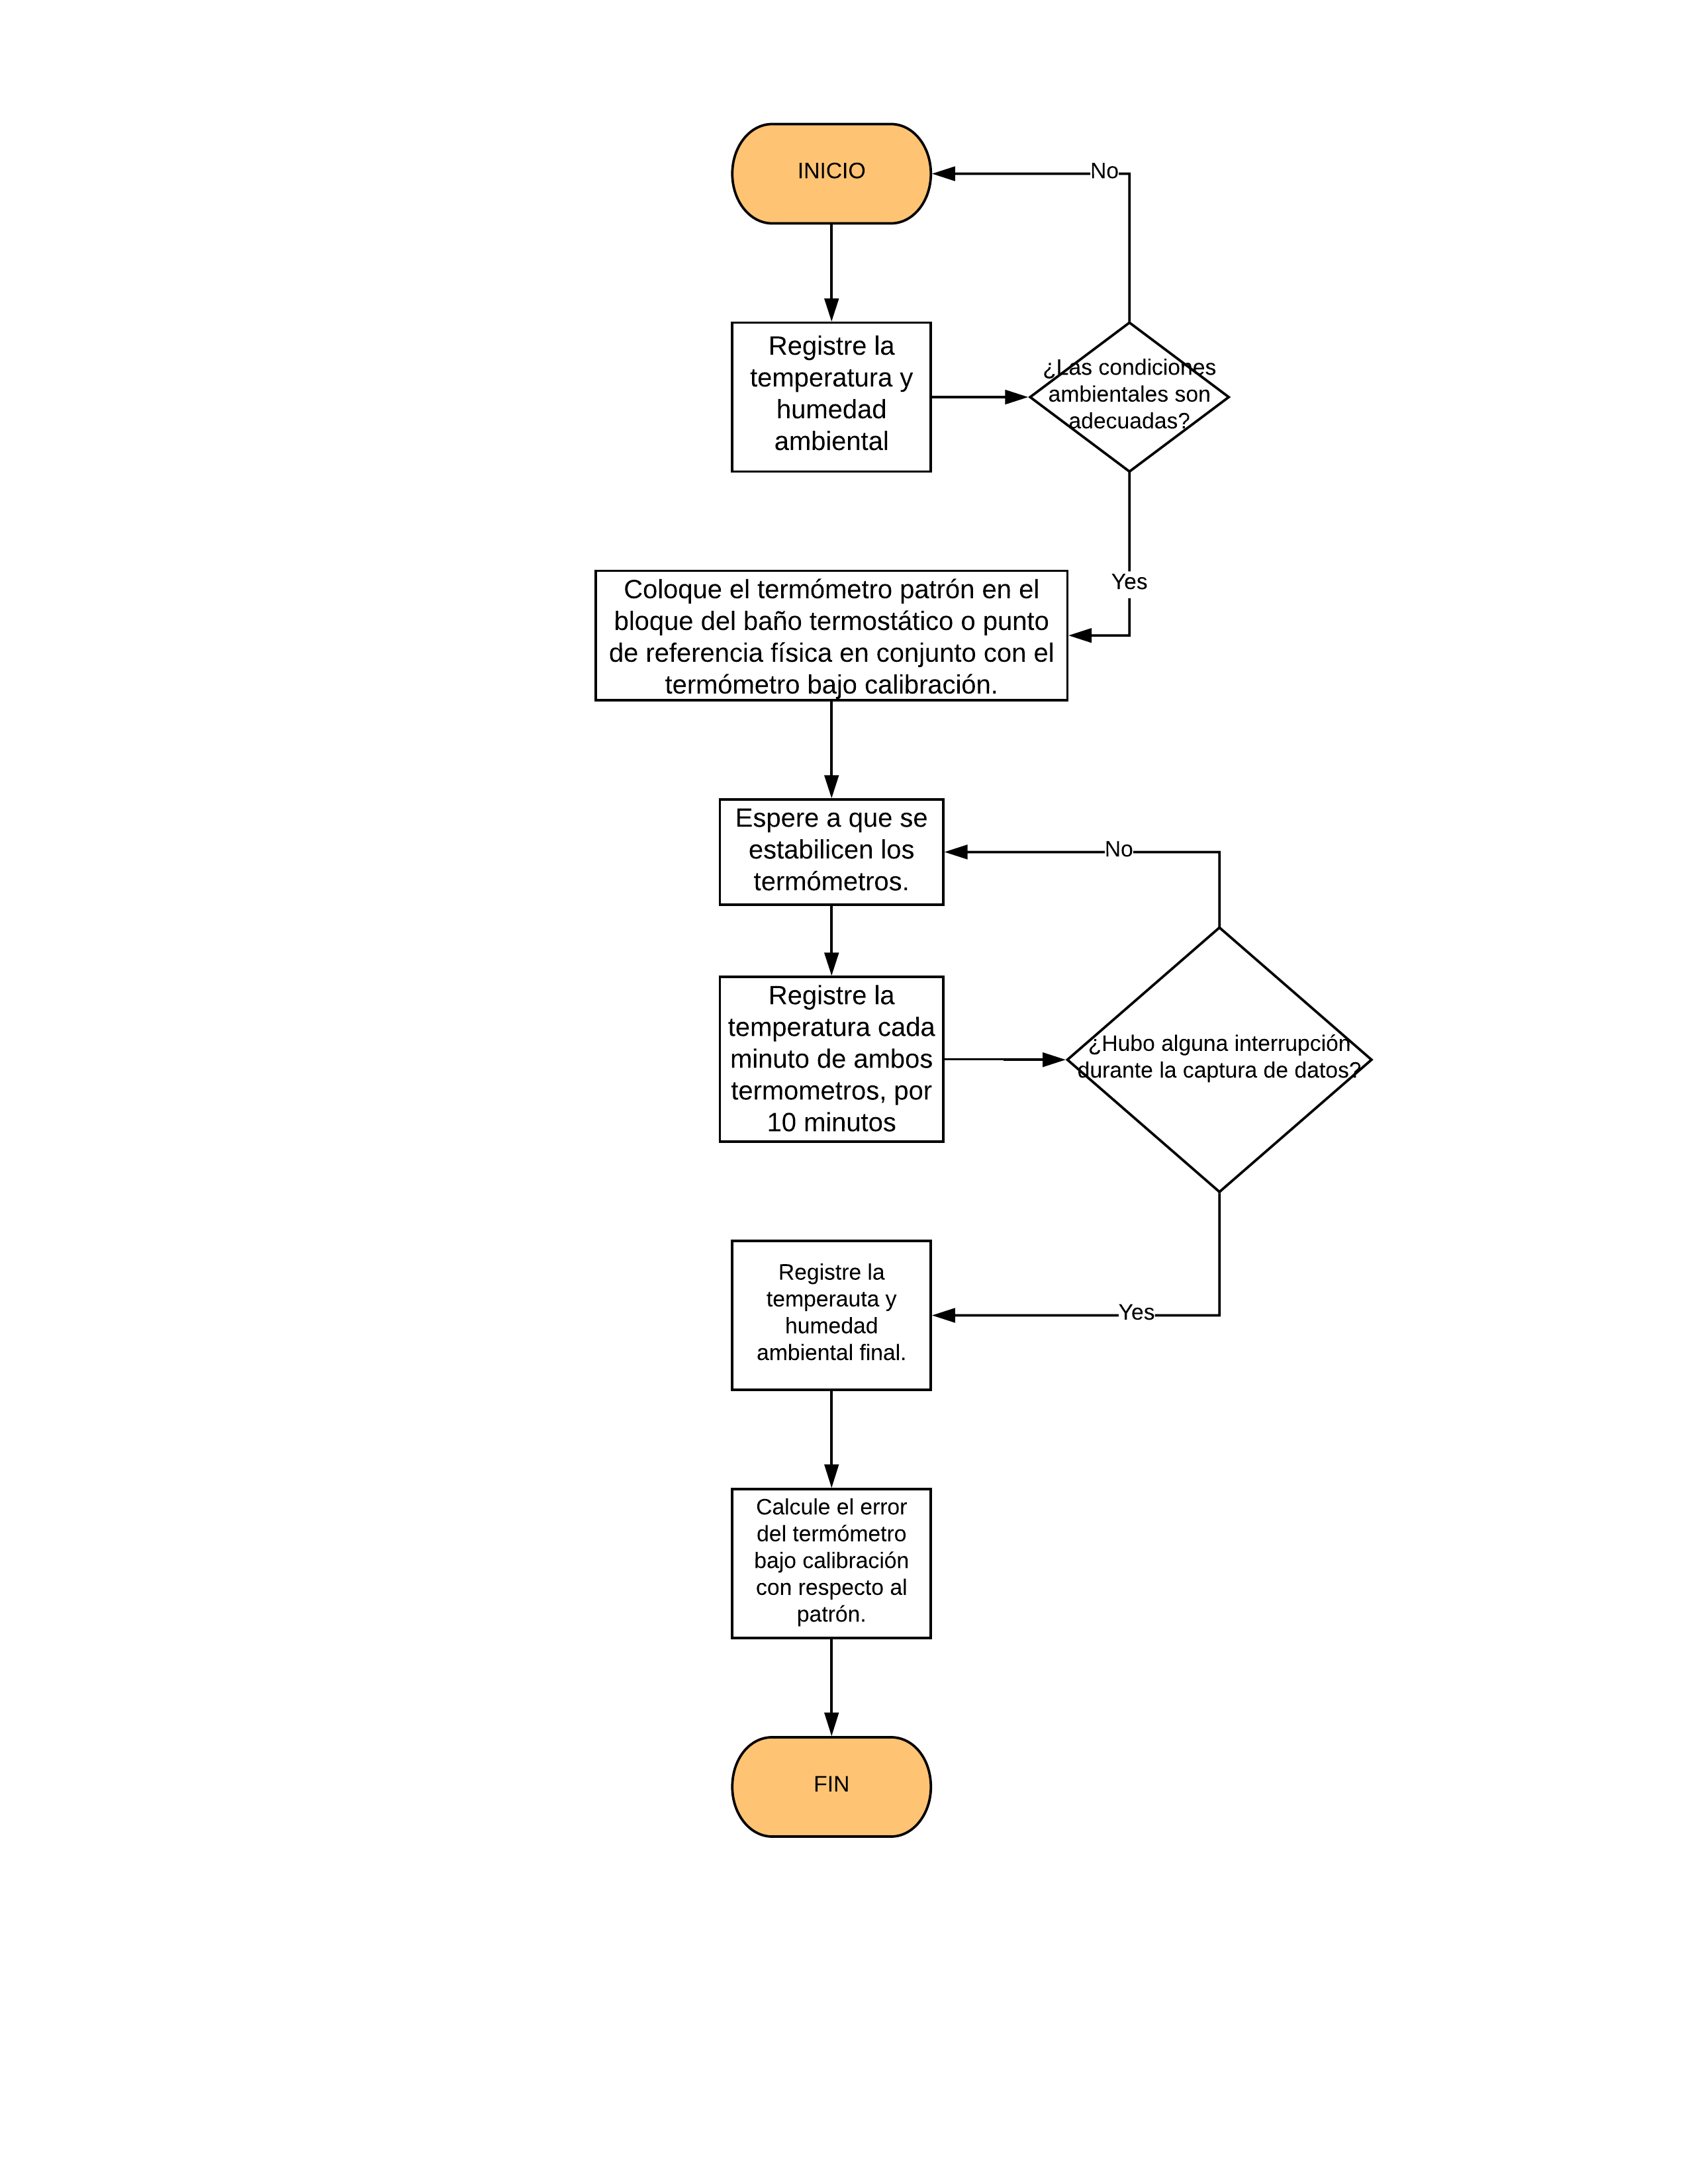
\includegraphics[width=\textwidth]{diagram2.png}
	\caption{Diagrama de Flujo del proceso operativo SIGCSA-PO-14}
\end{figure}

	
